% The Great Gatsby .tex
%-------------------------------------------------------------------------------
% Set Document
\documentclass[a4paper,12pt]{article}
%-------------------------------------------------------------------------------
% Packages
\usepackage{geometry}
\usepackage{graphicx}
\usepackage{amssymb}
\usepackage{float}
%-------------------------------------------------------------------------------
% Variables

%-------------------------------------------------------------------------------
% Fonts
%-------------------------------------------------------------------------------
% Document Head
\geometry{letterpaper}
\title{The Great Gatsby}
\author{F. Scott Fitzgerald}
\date{}
%-------------------------------------------------------------------------------
% Main Document
\begin{document}
\maketitle
\section{Chapter 1}

\begin{figure}[b!]
   \centering
     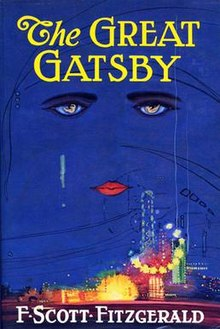
\includegraphics[width=0.25\textwidth]{images/jacket.jpg}
   \caption{The Great Gatsby}
\end{figure}

In my younger and more vulnerable years my father gave me some advice that I've been turning over in my mind ever since.

"Whenever you feel like criticising any one," he told me, "just
remember that all the people in this world haven't had the advantages
that you've had." \cite{my_cite_ref}

\bibliographystyle{plain}
\bibliography{bibliography/TheGreatGatsby.bib}
\end{document}
